\documentclass[11pt,a4paper]{book}
\usepackage{amsmath,amssymb}

\usepackage[utf8]{vietnam}
\usepackage{tikz}

\usepackage{mathabx}
\usepackage{amsmath}
\usepackage[left=1.5cm,right=1.5cm,top=0.67cm,bottom=2cm]{geometry}
\usepackage[dvips]{color} 
\usepackage{graphicx}
\usepackage{wrapfig}
\usepackage{scrextend}
\changefontsizes{12pt}
\usepackage{xcolor}
\usepackage{titlesec}
\usepackage{mdframed}
\renewcommand{\baselinestretch}{1.15}
\setlength{\parindent}{1pt}
\usepackage{fancyhdr}
\pagestyle{fancy}
\fancyhf{}
\lfoot{
\includegraphics[scale=0.1]{lg}\leftmark}
\rfoot{Trang \thepage/5 - Mã đề thi 209}

\usepackage{ex_test}
\renewcommand{\nameex}{\fontfamily{pag}\selectfont\color{teal} Câu}
\begin{document}
	\begin{minipage}[b]{0.355\textwidth}
		\centerline{\textbf{\fontsize{12}{0}\selectfont SỞ GD \& ĐT ĐỒNG THÁP}}
		\centerline{\textbf{TRƯỜNG THPT CHUYÊN}}
			\centerline{\textbf{ NGUYỄN QUANG DIÊU}}
		
		\centerline{(\textit{Đề thi có 04 trang})}
	\end{minipage}
	\begin{minipage}[b]{0.7\textwidth}
		\centerline{\textbf{\fontsize{12}{0}\selectfont KỲ THI THỬ TỐT NGHIỆP THPT NĂM 2021 LẦN I}}
		\centerline{\textbf{Bài thi: KHOA HỌC TỰ NHIÊN }}
		\centerline{\textbf{Môn thi thành phần: VẬT LÝ}}
		\centerline{\textit{\fontsize{12}{0}\selectfont Thời gian làm bài: 50 phút, không kể thời gian phát đề.}}
	\end{minipage}\\[0.1cm]
\rightline{
	\setlength\fboxrule{2pt} 
	\setlength\fboxsep{5pt} 
	\fbox{\textbf{Mã đề thi 209}}
}

\textbf{Họ và tên thí sinh:}................................................................\\ \textbf{Số báo danh:}...........................................................................



\begin{ex} 
Con lắc lò xo treo thẳng đứng, dao động điều hòa ở nơi có gia tốc trọng trường $g$. Khi vật ở vị trí cân bằng, độ dãn của lò xo là $\Delta \ell $  . Chu kỳ dao động của con lắc được tính bằng biểu thức
\choice 
{ $T=2\pi \sqrt{\dfrac{\Delta \ell }{g}}$ }
{  $T=\dfrac{1}{2\pi }\sqrt{\dfrac{m}{k}}$}
{ $T=\dfrac{1}{2\pi }\sqrt{\dfrac{g}{\Delta \ell }}$ }
{ $T=2\pi \sqrt{\dfrac{k}{m}}$  } \end{ex} 
\begin{ex} 
Quang phổ liên tục của một vật
\choice 
{ phụ thuộc vào nhiệt độ và bản chất của vật nóng sáng} 
{ phụ thuộc vào bản chất của vật nóng sáng} 
{ không phụ thuộc vào nhiệt độ của vật nóng sáng} 
{ phụ thuộc vào nhiệt độ của vật nóng sáng} \end{ex} 
\begin{ex} 
Công thoát của êlectron khỏi một kim loại là ${{6,625.10}^{-19}}\text{J}$. Biết $h={{6,625.10}^{-34}}\text{J}\text{.s}$,$c={{3.10}^{8}}\text{m/s}$. Giới hạn quang điện của kim loại này là
\choice 
{ 360 nm}
{ 350 nm}
{ 300 nm}
{ 260 nm} \end{ex} 
\begin{ex} 
Trong mạch xoay chiều $RLC$ nối tiếp. Biểu thức \textbf{không} đúng là:
\choice 
{ $i=\dfrac{{{u}_{L}}}{{{Z}_{L}}}$}
{ $i=\dfrac{{{u}_{R}}}{R}$}
{ $I=\dfrac{{{U}_{R}}}{R}$}
{ $I=\dfrac{{{U}_{L}}}{{{Z}_{L}}}$} \end{ex} 
\begin{ex} 
Cho một đoạn mạch $RLC$ nối tiếp. Biết $L=\dfrac{1}{\pi }$(H), $C=\dfrac{{{2.10}^{-4}}}{\pi }$(F), $R$ thay đổi được. Đặt vào hai đầu đoạn mạch một điện áp có biểu thức $u={{U}_0}\cos (100\pi t)$(V). Để $u_{C}$ chậm pha $\dfrac{3\pi }{4}$ so với $u$ thì $R$ phải có giá trị
\choice 
{ $R=50\Omega $}
{ $R=100\sqrt{2}\Omega $}
{ $R=100\Omega $}
{ $R=50\sqrt{2}\Omega $} \end{ex} 
\begin{ex} 
Biết khối lượng của proton, nơtron, hạt nhân $_{8}^{16}O$ lần lượt là 1,0073u; 1,0087u; 15,9904u và $1u=931,5MeV/{{c}^2}$. Năng lượng liên kết của hạt nhân $_{8}^{16}O$ xấp xỉ bằng:
\choice 
{ 128,17 MeV}
{ 190,81 MeV}
{ 14,25 MeV}
{ 18,76 MeV} \end{ex} 
\begin{ex} 
Phát biểu nào sau đây là \textbf{ không} đúng?
\choice 
{ Theo thuyết êlectron, một vật nhiễm điện dương là vật thiếu êlectron} 
{ Theo thuyết êlectron, một vật nhiễm điện âm là vật thừa êlectron} 
{ Theo thuyết êlectron, một vật nhiễm điện dương là vật đã nhận thêm các ion dương} 
{ Theo thuyết êlectron, một vật nhiễm điện âm là vật đã nhận thêm êlectron} \end{ex} 
\begin{ex} 
Hai điện tích điểm cùng độ lớn ${{10}^{-4}}$C đặt trong chân không, để tương tác nhau bằng lực có độ lớn ${{10}^{-3}}$ N thì chúng phải đặt cách nhau
\choice 
{ 90000 m}
{ 300 m}
{ 30000 m}
{ 900 m} \end{ex} 
\begin{ex} 
Hai âm có mức cường độ âm chênh lệch nhau là 40 dB. Tỉ số cường độ âm của chúng là
\choice 
{ ${{4.10}^3}$}
{ ${{10}^2}$}
{ ${{10}^4}$}
{ ${{4.10}^2}$} \end{ex} 
\begin{ex} 
Một sóng cơ có tần số $f$, truyền trên dây đàn hồi với tốc độ truyền sóng $v$ và bước sóng $\lambda $. Hệ thức đúng là
\choice 
{ $v=2\pi f\lambda $}
{ $v=\dfrac{\lambda }f$}
{ $v=\dfrac{f}{\lambda}$}
{ $v=\lambda f$} \end{ex} 
\begin{ex} 
Một học sinh làm thí nghiệm đo chu kì dao động của con lắc đơn. Dùng đồng hồ bấm giây đo 5 lần thời gian 10 dao động toàn phần lần lượt là 16,45 s; 16,10 s; 16,86 s; 16,25 s; 16,50 s. Bỏ qua sai số dụng cụ. Kết quả chu kì dao động là:
\choice 
{ $16,43s\pm 1,34\%$}
{ $1,64s\pm 0,21\%$}
	{ $16,43s\pm 0,21\%$}
		{ $1,64s\pm 1,28\%$} \end{ex} 
			\begin{ex} 
				Chọn câu đúng:
				\choice 
				{ Hiện tượng quang điện chứng tỏ ánh sáng có tính chất hạt} 
				{ Hiện tượng giao thoa chứng minh ánh sáng chỉ có tính chất hạt} 
				{ Khi bước sóng càng dài thì năng lượng phôtôn ứng với chúng càng lớn} 
				{ Tia hồng ngoại, tia tử ngoại không có tính chất hạt} \end{ex} 
			\begin{ex} 
				Một con lắc đơn có chiều dài dây treo $\ell =45$ cm, khối lượng vật nặng là $m=100$ (g). Con lắc dao động tại nơi có gia tốc trọng trường $g=10m/{{s}^2}$. Khi con lắc đi qua vị trí cân bằng, lực căng dây treo bằng 3 N. Tốc độ của vật nặng khi nó đi qua vị trí này là
				\choice 
				{ $3\sqrt{2}$ m/s}
				{ 2 m/s}
				{ 3 m/s}
				{ $3\sqrt{3}$  m/s} \end{ex} 
			\begin{ex} 
				Một dây đàn hồi rất dài có đầu $A$ dao động với tần số $f$ theo phương vuông góc với sợi dây. Tốc độ truyền sóng trên dây là 4 m/s. Xét điểm $M$ trên dây và cách $A$ một đoạn 14 cm, người ta thấy $M$ luôn dao động ngược pha với nguồn. Biết tần số $f$ có giá trị trong khoảng từ 98 Hz đến 102 Hz. Bước sóng của sóng đó có giá trị là
				\choice 
				{ 6 cm}
				{ 4 cm}
				{ 8 cm}
				{ 5 cm} \end{ex} 
			\begin{ex} 
				Trong thí nghiệm giao thoa ánh sáng người ta chiếu ánh sáng đơn sắc bước sóng $\lambda $ vào hai khe. Khoảng cách giữa hai khe là 0,5 mm. Khoảng cách giữa 11 vân sáng liên tiếp đo được là 1,2 cm. Nếu dịch chuyển màn ra xa hai khe thêm 30 cm thì đo được khoảng cách giữa 11 vân sáng liên tiếp là 1,5 cm. Bước sóng $\lambda $ bằng
				\choice 
				{ 500 nm}
				{ 750 nm}
				{ 600 nm}
				{ 450 nm} \end{ex} 
			\begin{ex} 
				Cho đoạn mạch điện $AB$ không phân nhánh mắc theo thứ tự: một cuộn cảm, một tụ điện có điện dung $C$ thay đổi được, một điện trở thuần $R=50\Omega $. Giữa $A,B$ có một điện áp xoay chiều luôn ổn định $u=164\sqrt{2}\cos \omega t$ (V). Cho $C$ thay đổi. Khi dung kháng của tụ điện bằng 40 $\Omega $ thì điện áp giữa hai đầu cuộn cảm lệch pha $\dfrac{\pi }{2}$ so với điện áp giữa hai đầu mạch $MB$ (mạch $MB$ chứa $C$ và $R$) và công suất tiêu thụ của mạch $AB$ lớn nhất ${{P}_{\max }}$. Giá trị của ${{P}_{\max }}$ bằng
				\choice 
				{ 537,92 (W)}
				{ 328 (W)}
				{ 672,5 (W)}
				{ 840,5 (W)} \end{ex} 
			\begin{ex} 
				Điều kiện để có sóng dừng trên dây khi khi một đầu dây cố định và đầu còn lại tự do là chiều dài $l$ của sợi dây phải thỏa mãn điều kiện
				\choice 
				{ $l=( 2k+1 )\dfrac{\lambda }{2}$}
				{ $l=k\dfrac{\lambda}{2}$}
				{ $l=( 2k+1 )\dfrac{\lambda }{4}$}
				{ $l=k \lambda $} \end{ex} 
			\begin{ex} 
					\immini{Cho mạch điện như hình vẽ: ${{R}_{1}}=1W,{{R}_{2}}=5W;{{R}_{3}}=12W;E=3V,r=1W$. Bỏ qua điện trở của dây nối.Hiệu suất của nguồn điện bằng
					\choice 
				{ 70 \%}
				{ 60 \%}
				{ 80 \%}
				{ 90 \%}		
				}{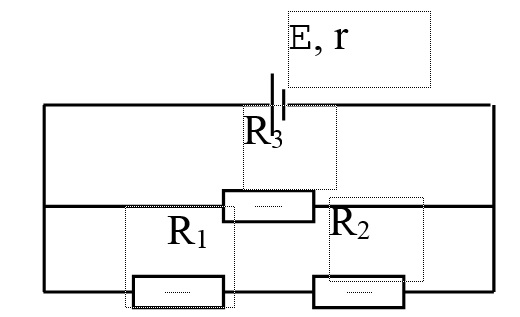
\includegraphics[scale=0.3]{c18}}
				
			 \end{ex} 
								\begin{ex} 
									Trong thí nghiệm Y-âng, nếu khoảng cách giữa hai vân sáng liên tiếp là $i$ thì vân tối thứ hai xuất hiện trên màn tại vị trí cách vân sáng trung tâm một khoảng bằng
									\choice 
									{ $i$}
									{ $2i$}
									{ $1,5i$}
									{ $0,5i$} \end{ex} 
								\begin{ex} 
									Một vật thực hiện đồng thời hai dao động điều hòa cùng phương, cùng tần số có biên độ lần lượt là 8 cm và 12 cm. Biên độ dao động tổng hợp có thể là
									\choice 
									{ $A=21$ cm}
									{ $A=3$ cm}
									{ $A=2$ cm}
									{ $A=5$ cm
								} \end{ex} 
								\begin{ex} 
									Tia $X$ cứng và tia $X$ mềm có sự khác biệt về
									\choice 
									{ bản chất và bước sóng} 
									{ năng lượng và tần số} 
									{ bản chất và năng lượng} 
									{ bản chất, năng lượng và bước sóng} \end{ex} 
								\begin{ex} 
									Một máy phát điện xoay chiều một pha có rôto là phần cảm, cần phát ra dòng điện có tần số không đổi 60 Hz để duy trì hoạt động của một thiết bị kỹ thuật. Nếu thay rôto của máy phát điện bằng một rôto khác có ít hơn hai cặp cực thì số vòng quay của rôto trong một giờ phải thay đổi đi 18000 vòng. Số cặp cực của rôto lúc đầu là
									\choice 
									{ 6}
									{ 10}
									{ 4}
									{ 5} \end{ex} 
								\begin{ex} 
									Khi nói về tia $\alpha $, phát biểu nào dưới đây là đúng?
									\choice 
									{ Trong chân không, tia $\alpha $ có vận tốc bằng ${{3.10}^{8}}$m/s} 
									{ Tia $\alpha $ có khả năng ion hóa không khí} 
									{ Tia $\alpha $là dòng các hạt trung hòa về điện} 
									{ Tia $\alpha $ là dòng các hạt prôtôn} \end{ex} 
								\begin{ex} 
									Khi bắn phá hạt nhân ${}_{7}^{14}N$ bằng hạt $\alpha $, người ta thu được một hạt prôtôn và một hạt nhân $X$. Hạt nhân $X$ là
									\choice 
									{ ${}_{6}^{12}C$}
									{ ${}_{8}^{17}O$}
									{ ${}_{8}^{16}O$}
									{ ${}_{6}^{14}C$} \end{ex} 
								\begin{ex} 
									Một vật dao động tắt dần có các đại lượng giảm liên tục theo thời gian là
									\choice 
									{ li độ và tốc độ}
									{ biên độ và tốc độ} 
									{ biên độ và năng lượng}
									{ biên độ và gia tốc} \end{ex} 
								\begin{ex} 
									Một mạch dao động lí tưởng gồm cuộn cảm thuần có độ tự cảm $L$ không đổi và tụ điện có điện dung $C$ thay đổi được. Điều chỉnh điện dung của tụ điện đến giá trị ${{C}_{1}}$ thì tần số dao động riêng của mạch là ${f_{1}}$. Để tần số dao động riêng của mạch là ${f_{ & 1}}\sqrt[]{5}$ thì phải điều chỉnh điện dung của tụ điện đến giá trị
									\choice 
									{ $\sqrt[]{5}{{C}_{1}}$}
									{ $5{{C}_{1}}$}
									{ $\dfrac{{{C}_{1}}}{\sqrt{5}}$}
									{ $\dfrac{{{C}_{1}}}{5}$ } \end{ex} 
								\begin{ex} 
									Cường độ dòng điện không đổi được xác định bằng công thức nào sau đây?
									\choice 
									{ $I=\dfrac{t}{q}$}
									{ $I=q.t$}
									{ $I=\dfrac{q}e$}
									{ $I=\dfrac{q}{t}$} \end{ex} 
								\begin{ex} 
									Hai bóng đèn có các hiệu điện thế định mức lần lượt là ${{U}_{1}}$ và ${{U}_{2}}$. Nếu công suất định mức của hai bóng đó bằng nhau thì tỷ số hai điện trở ${{R}_{1}}/{{R}_{2}}$ là
									\choice 
									{ $\dfrac{{{U}_{2}}}{{{U}_{1}}}$  }
									{ ${{( \dfrac{{{U}_{2}}}{{{U}_{1}}} )}^2}$}
									{ $\dfrac{{{U}_{1}}}{{{U}_{2}}}$  }
									{ ${{( \dfrac{{{U}_{1}}}{{{U}_{2}}} )}^2}$} \end{ex} 
								\begin{ex} 
									Trong hiện tượng giao thoa sóng nước, hai nguồn $A,B$ cách nhau 20 cm dao động cùng biên độ, cùng pha, cùng tần số 50 Hz. Tốc độ truyền sóng trên mặt nước là 1,5 m/s. Xét trên đường thẳng d vuông góc với $AB$ và cách trung trực của $AB$ một khoảng 7 cm, điểm dao động cực đại trên $d$ và gần $A$ nhất cách $A$ một khoảng là
									\choice 
									{ 5,67 cm}
									{ 8,75 cm}
									{ 10,64 cm}
									{ 14,46 cm} \end{ex} 
								\begin{ex} 
									Hệ số công suất của một đoạn mạch xoay chiều gồm $R,L,C$ ghép nối tiếp được tính bởi công thức:
									\choice 
									{ $\cos \varphi =\dfrac{{{Z}_{C}}}{Z}$}
									{ $\cos \varphi =\dfrac{R}{Z}$}
									{ $\cos \varphi =\dfrac{{{Z}_{L}}}{Z}$}
									{ $\cos \varphi =RZ$
								} \end{ex} 
							\newpage
								\begin{ex} 
									
										\immini{Đặt một điện áp $u={{U}_0}\cos \omega t$ (${{U}_0},\omega $ không đổi) vào hai đầu đoạn mạch $RLC$ nối tiếp. Cho biết $R=100\Omega $ cuộn cảm thuần có độ tự cảm $L$ thay đổi được. Hình bên là đồ thị biểu diễn sự phụ thuộc của công suất tiêu thụ điện của đoạn mạch theo độ tự cảm $L$. Dung kháng của tụ điện là
										\choice 
									{ $100\Omega $}
									{ $200\Omega $}
									{ $150\Omega $}
									{ $100\sqrt{2}\Omega $}	
											
									}{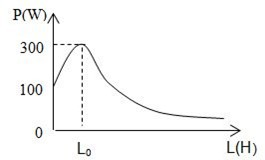
\includegraphics[scale=0.7]{c31}}
								 \end{ex} 
								\begin{ex} 
									Trong mạch dao động $LC$ lý tưởng, gọi ${{Q}_0}$ là điện tích cực đại của tụ điện; ${{I}_0}$ là cường độ dòng điện cực đại trong mạch. Chu kỳ dao động riêng của mạch là
									\choice 
									{ $2\pi \dfrac{{{Q}_0}}{{{I}_0}}$}
									{$\dfrac{{{I}_0}}{2\pi {{Q}_0}}$}
									{ $2\pi \dfrac{{{I}_0}}{{{Q}_0}}$}
									{ $\dfrac{{{Q}_0}}{2\pi {{I}_0}}$} \end{ex} 
								\begin{ex} 
									Trong thí nghiệm young về giao thoa ánh sáng, nguồn $S$ phát ra ba ánh sáng đơn sắc: ${{\lambda }_{1}}=0,42\mu m$(màu tím), ${{\lambda }_{2}}=0,56\mu m$(màu lục) và ${{\lambda }_{3}}=0,70\mu m$(màu đỏ). Giữa hai vân sáng liên tiếp có màu giống như màu của vân trung tâm có
									\choice 
									{ 6 vạch màu đỏ}
									{ 19 vạch màu tím}
									{ 44 vạch sáng}
									{ 14 vạch màu lục} \end{ex} 
								\begin{ex} 
									Cơ năng của một chất điểm dao động điều hòa tỉ lệ thuận với
									\choice 
									{ biên độ dao động}
									{ bình phương biên độ dao động} 
									{ li độ của vật}
									{ chu kỳ dao động} \end{ex} 
								\begin{ex} 
									Đơn vị cường độ	 âm có thể là
									\choice 
									{ dB}
									{ $W/{{m}^2}$}
									{ m/s}
									{ m} \end{ex} 
								\begin{ex} 
									Electron quang điện khi bật ra khỏi kim loại thì bay vào từ trường đều với cảm ứng từ $B={{10}^{-5}}T$ theo quỹ đạo tròn mà hình chiếu của electron trên một đường kính sẽ dao động điều hòa với biên độ 10 cm. Cho khối lượng electron là ${{9,1.10}^{-31}}kg$ và điện tích electron là $-{{1,6.10}^{-19}}C$. Vận tốc electron có độ lớn là:
									\choice 
									{ ${{3,52.10}^{6}}$ m/s}
									{ ${{3,52.10}^5}$ m/s}
									{ ${{1,76.10}^{6}}$ m/s}
									{ ${{1,76.10}^5}$ m/s} \end{ex} 
								\begin{ex} 
									Máy biến áp được dùng để
									\choice 
									{ Biến đổi dòng ðiện xoay chiều thành dòng điện một chiều} 
									{ Thay đổi tần số dòng điện} 
									{ Biến đổi dòng điện một chiều thành dòng điện xoay chiều} 
									{ Thay đổi điện áp xoay chiều} \end{ex} 
								\begin{ex} 
									So với hạt nhân ${}_{14}^{29}Si$  , hạt nhân ${}_{20}^{40}Ca$  có nhiều hơn
									\choice 
									{ 11 nơtrôn và 6 prôtôn}
									{ 6 nơtrôn và 5 prôtôn} 
									{ 5 nơtrôn và 6 prôtôn}
									{ 5 nơtrôn và 12 prôtôn} \end{ex} 
								\begin{ex} 
									Một vật dao động điều hòa dọc theo trục $Ox$. Mốc thế nắng ở vị trí cân bằng. Ở thời điểm độ lớn vận tốc của vật bằng 50\% vận tốc cực đại thì tỉ số giữa động năng và cơ năng của vật là
									\choice 
									{ 1/2}
									{ 1/4}
									{ 4/3}
									{ 3/4} \end{ex} 
								\begin{ex} 
									Phát biểu nào sau đây về tính chất của sóng điện từ là \textbf{không} đúng?
									\choice 
									{ Sóng điện từ có thể phản xạ, khúc xạ, giao thoa} 
									{ Sóng điện từ mang năng lượng} 
									{ Sóng điện từ truyền trong chân không với tốc độ nhỏ nhất} 
									{ Sóng điện từ là sóng ngang.} \end{ex}
								\textbf{\begin{center}
		------------------ HẾT ------------------\\
			\textbf{	\textit{Thí sinh không được sử dụng tài liệu. Cán bộ coi thi không giải thích gì thêm}}
		
\end{center}}

\end{document}
